%----------------Cap_02----------------%

\chapter{O MODELO DE DISSERTAÇÃO PROFMAT/UFT}


O código-fonte deste modelo está disponível no link \url{https://pt.sharelatex.com/project/55391d40527ca0810cb26f82}\footnote{Como este modelo também pode ser usado como um manual básico de latex, é aconselhável que o mestrando salve uma cópia em local reservado antes de fazer alterações no código-fonte.}. Sugere-se que o mestrando possua uma conta na plataforma Overleaf. Nesse caso, terá acesso imediato a uma cópia do modelo para elaboração de sua dissertação, conforme mostrado na Figura

\begin{figure}[H]
    \centering
    \caption{Modelo de dissertação PROFMAT/UFT na plataforma Overleaf}
    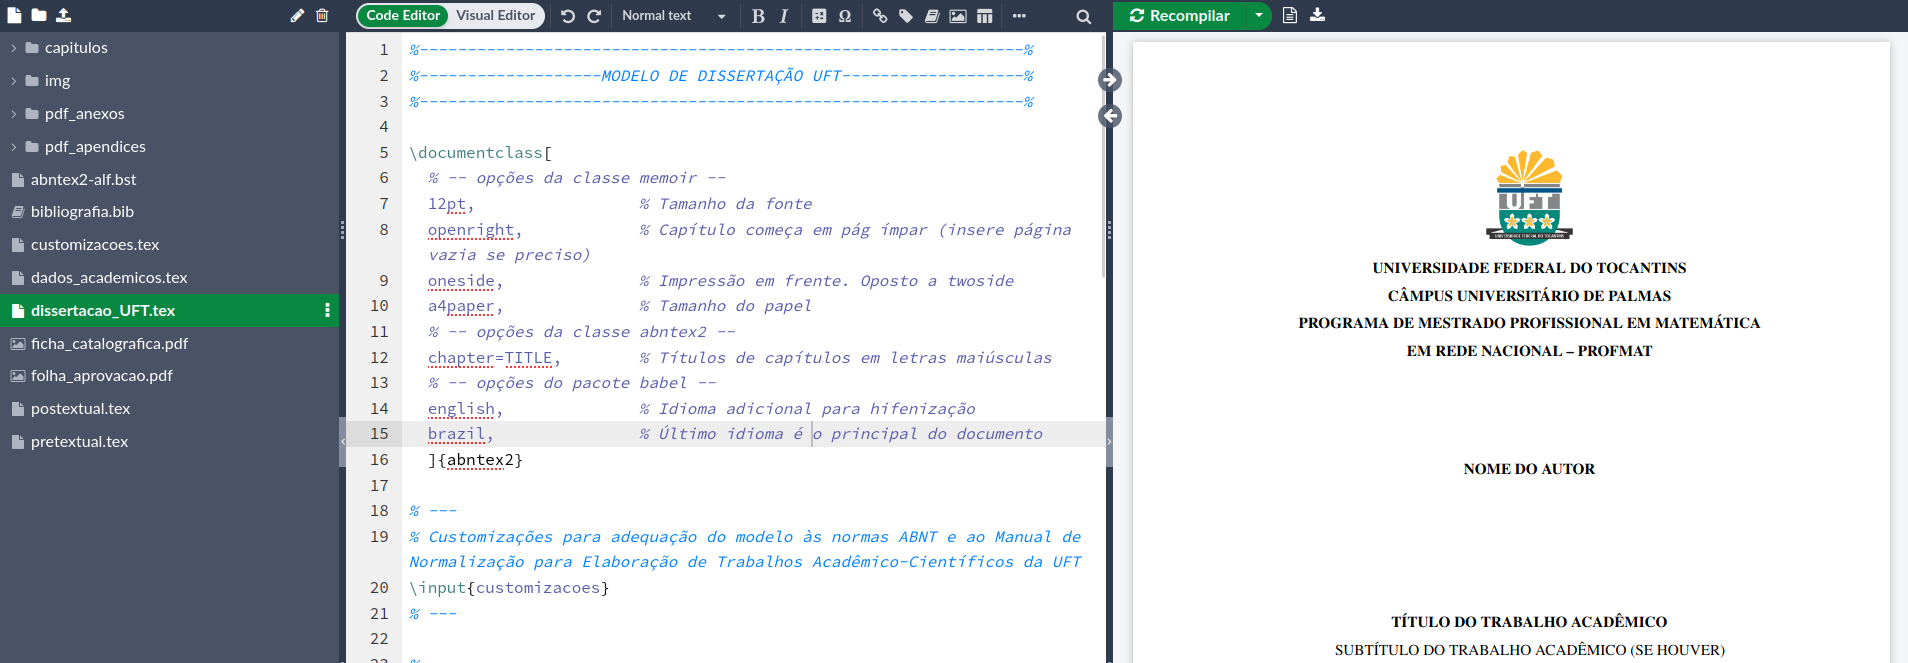
\includegraphics[width=\textwidth]{img/modelo_dissertacao_01.png}
    \label{fig:modelo_dissertacao_01}
\end{figure}





Os arquivos serão baixados dentro de uma pasta zipada. Para abrí-los, é necessário o uso de programas descompactadores como \textit{winrar} ou \textit{7-zip}. Então, basta extrair os arquivos dentro de uma pasta onde possam ser alterados, conforme sequência detalhada a seguir.

Basicamente, a pasta conterá um arquivo principal (doravante chamado arquivo mestre) com o nome \textbf{Dissertacao\_UFT.tex}. Este arquivo conterá a estrutura fundamental da dissertação como os comandos de formatação geral do trabalho, dados do aluno, nome do orientador, título da dissertação, dentre outros.

O arquivo \textbf{Pretextual.tex} contém os comandos para criação dos elementos pré-textuais da dissertação (capa, folha de rosto, folha de aprovação, resumo, etc.). 

Cada capítulo do modelo de dissertação está escrito em um dos arquivos: \textbf{Cap\_01.tex, Cap\_02.tex, Cap\_03.tex}, etc. que correspondem ao desenvolvimento do trabalho desde a introdução até a conclusão. 

O arquivo  \textbf{Postextual.tex} contém os comandos para criação das referências bibliográficas bem como alguns modelos de apêndices e anexos que possam ser úteis para o trabalho. 

Os arquivos listados acima devem estar salvos na mesma pasta em que se encontra o arquivo mestre. Cada um deles é escrito separada e independentemente dos demais. A adição destes arquivos ao  arquivo mestre é feita com o uso do comando: 
\begin{verbatim}
\include{nome-do-arquivo}
\end{verbatim}
executado no arquivo mestre.

Além destes arquivos, a pasta contém alguns modelos em PDF para a ficha de aprovação (\textbf{FichadeAprovacao.pdf}), para a ficha catalográfica  (\textbf{FichaCatalografica.pdf}), para um apêndice em PDF (\textbf{Apendice.pdf}), um anexo em PDF (\textbf{Anexo.pdf}) e uma pasta onde mestrando deverá salvar todas as figuras e ilustrações que irá inserir em seu trabalho.

\section{Inserindo dados no arquivo mestre}

Assim que abrir o arquivo \textbf{Dissertacao\_UFT.tex} em um editor LaTeX\footnote{Sugere-se o uso do editor TexMaker \cite{texmaker-org} para sistema operacional Windows.}, o leitor irá se deparar com os comandos gerais para a formatação de seu trabalho escritos no \textbf{preâmbulo} do arquivo onde, logo no início é possível visualizar a \textbf{classe} escolhida para o documento, os pacotes utilizados, bem como as customizações realizadas para que o modelo atendesse plenamente às normas ABNT.

Ao final do arquivo \textbf{Dissertacao\_UFT.tex}, o aluno encontrará os seguintes campos para preenchimento das principais informações da dissertação: Nome do Autor, Título e Subtítulo, Orientador, dentre outras.
\begin{verbatim}
% ---
% Informações do Trabalho a serem informadas pelo AUTOR
% ---
\titulo{Título do Trabalho Acadêmico}

\subtitulo{Subtítulo do Trabalho Acadêmico (Se Houver)}   
% Caso não haja subtítulo, basta apagar a linha acima.

\autor{Nome do Autor}

\orientador{Prof. Dr. ``Nome do Orientador''}

\examinadorA{Prof. Dr. ``Nome do examinador A''}

\examinadorB{Prof. Dr. ``Nome do examinador B''}

\instituicao{Universidade Federal do Tocantins}

\campus{Palmas}

\data{20XX}

\tipotrabalho{Dissertação (Mestrado)}

% O preambulo deve conter o tipo do trabalho, o objetivo, 
% o nome da instituição e a área de concentração 
\preambulo{Dissertação apresentado ao Programa de Mestrado Profissional 
em Matemática em Rede Nacional - PROFMAT da Universidade Federal do 
Tocantins como requisito parcial para a obtenção do título de 
Mestre - Área de Concentração: Matemática.\\
Orientador: \imprimirorientador.}
% ---
\end{verbatim}

Após o preenchimento desses campos, a capa, folha de rosto e folha de aprovação serão automaticamente atualizadas com os dados da dissertação.


A estrutura do trabalho é dividida em três partes, a saber:
\begin{itemize}
	\item \textbf{Elementos pré-textuais};
	\item \textbf{Elementos textuais};
	\item \textbf{Elementos pós-textuais}.
\end{itemize}
sendo que cada um destes elementos encontra-se em um dos arquivos (com extensão .tex) já descritos na seção anterior.


Para finalizar esta seção, um comentário sobre o comando \verb!\include{}!. Para compilar todos os arquivos simultaneamente, estes devem estar no arquivo mestre como mostrado abaixo


Como afirmado acima, o comando \verb!\include{}! permite escrever separadamente cada parte do documento, por exemplo, cada capítulo. Isto é especialmente vantajoso em se tratando de documentos grandes. Por exemplo, quando se está trabalhando no capítulo 1 (arquivo \textbf{Cap\_01.tex}), é possível desativar a compilação dos demais arquivos. Para isso, basta inserir o comando  \verb!%! a direita da cada \verb!\include{}! não utilizado. No caso deste exemplo, no arquivo mestre, ter-se-ia:

\begin{verbatim}
%\include{Cap_01}

\include{Cap_02}

%\include{Cap_03}

%\include{Cap_04}

%\include{Cap_05}
\end{verbatim}

Além de tornar o trabalho mais organizado, isso diminui o tempo de compilação\footnote{Processo por meio do qual o programa editor de LaTeX interpreta os comandos escritos no código-fonte e converte-os em um arquivo final e pronto para impressão ou leitura na tela do computador.} do documento (já que o computador só irá compilar a parte do documento que está ativa) e facilita a busca de erros que possam ocorrer (pois toda a atenção do autor estará concentrada apenas em uma parte do documento).

Ao final, basta remover os símbolos \verb!%! a direita do comando \verb!\include{}! e compilar o documento inteiro.

\section{Elementos pré-textuais}

O arquivo \textbf{Pretextual.tex} é responsável pela impressão da capa e pela inclusão dos elementos pré-textuais da dissertação. Conforme NBR 14724/2011 \cite{nbr14724}, os elementos pré-textuais são
\begin{itemize}
	\item Folha de rosto (obrigatório);
	\item Errata (opcional);
	\item Folha de aprovação (obrigatório);
	\item Dedicatória (opcional);
	\item Agradecimentos (opcional);
	\item Epígrafe (opcional);
	\item Resumo na língua vernácula (obrigatório);
	\item Resumo em língua estrangeira (obrigatório);
	\item Lista de ilustrações (opcional);
	\item Lista de tabelas (opcional);
	\item Lista de abreviaturas e siglas (opcional);
	\item Lista de símbolos (opcional);
	\item Sumário (obrigatório).
\end{itemize}

Com exceção da errata, este modelo contém todos os elementos listados. Conforme a necessidade, pode-se descartar um ou mais elementos opcionais. Por exemplo, se não há necessidade de uma dedicatória, basta apagar do arquivo \textbf{Pretextual.tex} os comandos:
\begin{verbatim}
%----------------------Dedicatória----------------------%
\begin{dedicatoria}
\vspace*{\fill}
	\begin{flushright}
		\textit{A Fulano.\\
   		A Beltrano.}
	\end{flushright}
\end{dedicatoria}
\end{verbatim}

A respeito da \textbf{ficha catalográfica}, este modelo de dissertação inclui comandos para uma ficha temporária, entre os comandos
\begin{verbatim}
\begin{fichacatalografica}
	\vspace*{\fill}					% Posição vertical
	\hrule							% Linha horizontal
\end{verbatim}
\qquad \qquad \vdots \quad \vdots \quad \vdots
\begin{verbatim}
	\end{minipage}
	\end{center}
	\hrule
\end{fichacatalografica}
\end{verbatim}

Obviamente, esta ficha temporária não possui validade. Portanto, assim que aprovada a dissertação, o mestrando irá solicitar junto a biblioteca do câmpus a definitiva ficha catalográfica para seu trabalho. Quando estiver com o documento, salve-o como PDF com o nome \textbf{FichaCatalografica} (tal como escrito aqui) no mesmo diretório do seu projeto, apague os comandos da ficha temporária e ative o comando abaixo:
\begin{verbatim}
\begin{fichacatalografica}
	\includepdf{FichaCatalografica.pdf}
\end{fichacatalografica}
\end{verbatim}

O mesmo ocorre com a \textbf{folha de aprovação}. Este modelo apresenta um modelo temporário de folha de aprovação.

Esse modelo encontra-se em conformidade com o \textbf{Manual de normalização para elaboração de trabalhos acadêmico-científicos da Universidade Federal do Tocantins} \cite{ManualUFT}. 

Portanto, assim que defendida e aprovada a dissertação, o mestrando irá receber um documento assinado pelos professores que compõem a banca de avaliação. Após isso, deve-se substituir os comandos 
\begin{verbatim}
%----------------------Folha de Aprovação----------------------%
\begin{folhadeaprovacao}
    \begin{center}
        \MakeUppercase{\imprimirautor}\\
        \vspace{1.5cm}
        \MakeUppercase{\textbf{\imprimirtitulo}} \\
        \MakeUppercase{\imprimirsubtitulo}\\
        \vspace{2.5cm}
    \end{center}
    \hspace{.45\textwidth}
    \begin{minipage}{.5\textwidth}
        \SingleSpacing
        \imprimirpreambulo
    \end{minipage}
   
   \vspace{2.5cm}
   
    \noindent Data de Aprovação: \noindent \hspace{0.1cm} \rule{0.75cm}{0.4pt} / \rule{0.75cm}{0.5pt} / \rule{1.2cm}{0.5pt}
    \vspace{1.5cm}
    
    \noindent Banca examinadora:
    \assinatura{\imprimirorientador, Orientador(a), UFT} 
    \assinatura{\imprimirexaminadorA, Examinador(a), UFT}
    \assinatura{\imprimirexaminadorB, Examinador(a), IFTO}
\end{folhadeaprovacao}
\end{verbatim}
por um arquivo PDF (nomeado conforme abaixo) da folha assinada pela banca, por meio do comando:
\begin{verbatim}
\includepdf{FichadeAprovacao.pdf}
\end{verbatim}

Os demais elementos do arquivo \textbf{Pretextual.tex} serão preenchidos pelo autor de acordo com as orientações no próprio arquivo. 

A \textbf{lista de ilustrações}, a \textbf{lista de tabelas} e o \textbf{sumário} são construídos automaticamente a medida que o autor insere figuras, tabelas ou tópicos (capítulos, seções, subseções, etc.) ao documento.

\section{Elementos textuais}

Ainda sobre a estrutura dos trabalhos acadêmicos, a norma NBR 14724/2011  prescreve que ``o texto é composto de uma parte introdutória, que apresenta os objetivos do trabalho e as razões de sua elaboração; o desenvolvimento, que detalha a pesquisa ou estudo realizado; e uma parte conclusiva''\cite[p.~8]{nbr14724}.

Neste modelo, são reservados os arquivos \textbf{Cap\_01.tex, Cap\_02.tex, Cap\_03.tex}, etc. para a escrita de cada capítulo da dissertação.

\section{Elementos pós-textuais}

No arquivo \textbf{Postextual.tex}, encontram-se os comandos para a criação das referências utilizadas durante a pesquisa e para a confecção de apêndices ou anexos, conforme a necessidade.

À medida que o autor da dissertação insere citações no corpo do texto, as referências são automaticamente criadas em local apropriado do arquivo por meio do comando
\begin{verbatim}
\bibliography{bibliografia}
\end{verbatim}

Maiores detalhes sobre este tema serão fornecidos em tópico especifico tratando a respeito de citações e referências. De acordo com a norma \citeonline{nbr14724}, apêndices e anexos são elementos opcionais. Caso não haja necessidade destes itens, basta removê-los do arquivo \textbf{Postextual.tex}.